\documentclass{article}
\usepackage[utf8]{inputenc}
\usepackage{listings}
\usepackage{graphicx}
\usepackage{hyperref}
\usepackage{float}
\usepackage[titletoc,title]{appendix}

\lstset{
  language=R,                 % the language of the code
  basicstyle=\footnotesize,        % the size of the fonts that are used for the code
  breaklines=true,                 % sets automatic line breaking
  extendedchars=true,              % lets you use non-ASCII characters; for 8-bits encodings only, does not work with UTF-8
  frame=single,	                   % adds a frame around the code
  keepspaces=true,                 % keeps spaces in text, useful for keeping indentation of code (possib
  otherkeywords={*,...},           % if you want to add more keywords to the set
  numbers=left,                    % where to put the line-numbers; possible values are (none, left, right)
  numbersep=5pt,                   % how far the line-numbers are from the co
  showstringspaces=false,          % underline spaces within strings only
  showtabs=false,                  % show tabs within strings adding particular underscores
  tabsize=2,	                   % sets default tabsize to 2 spaces
}

\title{Cognitive Modeling - Assignment 4: Yazayeri}
\author{Steven Bosch (s1861948)}

\begin{document}
\maketitle

\section{Code}
The following code gives my implementation for the readySetGo experiment. I used two more files, time.R and DM-module.R, which can be found in the appendix.
\lstinputlisting{Assignment4_Yazayeri.R}

\section{Plots}
This code yields the graph given in figure \ref{fig1}, modelling 6 subjects doing 1000 trials per condition, after having done 500 training trials.

\begin{figure}[H]
	\centering
	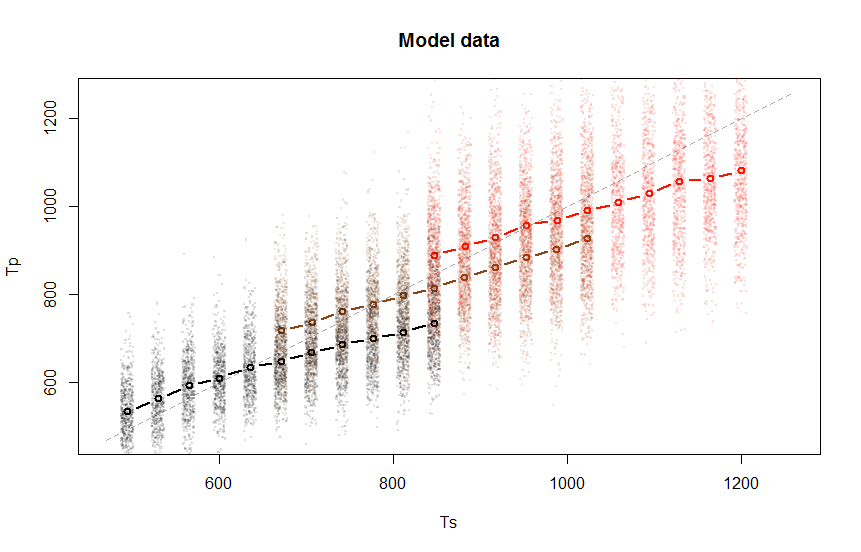
\includegraphics[width=\textwidth]{1.png}
	\caption{Interval estimation in the readySetGo experiment, using a cognitive model that ran for 6 subjects doing 1000 trials per condition after 500 training trials.}
	\label{fig1}
\end{figure}

\begin{appendices}
	\section{Code}
	\lstinputlisting[caption={time},label={time}]{time.R}
	\lstinputlisting[caption={DM-module},label={DM}]{DM-module.R}
\end{appendices}
\end{document}
